

\documentclass{sig-alternate-05-2015}

% Include useful packages
\usepackage{graphicx}
\graphicspath{ {images/} }
\usepackage{float}


\begin{document}

% Copyright
\setcopyright{acmcopyright}

\title{Approaches to Incorporating Whole Genome and Multi-Omics Information in the context of Clincal Prediction}

\author{
% You can go ahead and credit any number of authors here,
% e.g. one 'row of three' or two rows (consisting of one row of three
% and a second row of one, two or three).
%
% The command \alignauthor (no curly braces needed) should
% precede each author name, affiliation/snail-mail address and
% e-mail address. Additionally, tag each line of
% affiliation/address with \affaddr, and tag the
% e-mail address with \email.
%
% 1st. author
Siddharth Avadhanam\\
       \email{avadhana@msu.edu}
}
% There's nothing stopping you putting the seventh, eighth, etc.
% author on the opening page (as the 'third row') but we ask,
% for aesthetic reasons that you place these 'additional authors'
% in the \additional authors block, viz.
\date{\today}
% Just remember to make sure that the TOTAL number of authors
% is the number that will appear on the first page PLUS the
% number that will appear in the \additionalauthors section.

\maketitle



\section{Problem Description}

The high-dimensionality and complexity of data coming in from Genome Wide Association Studies
poses a whole range of statistical and computational challenges in finding genetic covariates of important phenotypes
( disease, yield , height etc). These data commonly contain thousands of individuals with information on
hundreds of thousands of markers. \cite{zhang_chapter_2012} An important issue which has been given considerable attention in the statistical genetics
literature is how to choose a subset of these markers so that the analysis of these data with standard commodity hardware and statistical methods
becomes more tractable.\cite{de_los_campos_whole-genome_2013} Methods which analyze a single-marker at a time are popular, but are severly limited in that they do not take into account
interactions between markers, and come with their own set of challenges related to multiple testing.\cite{moskvina_multiple-testing_2008}
It is thus becoming increasingly important to explore methods that incorporate information form the whole genome and possibly from outside the domain of traditional statistics.

Further, while methods that incorporate information form the whole genome simultaneously are finding increasing success, there is only so much that can be accomplished by solely considering genetic marker information.
These apporaches as a whole are running into the problems of missing heritability and are able to explain only a small proportion of the inter-individual variation for multifactorial outcomes such as height.\cite{eichler_missing_2010}
The complexity of the underlying biology demands approaches that can synthesize data from multiple platforms and consider factors contributing to disease that lie outside the genome. This more biologically realistic approach
would include data sources as diverse as epigenetics, pedigree data, transcriptomic data,  proteomic data etc.\cite{kim_multi-omics_2016} Here we will consider incorporating epigenetic and pedigree data in addition to genomic data.

Finally, we will be considering Kernel based approaches within and outside of the bayesian paradigm
and how they can be applied to genomic enabled clinical prediction. Kernel methods have immense flexibility ( can be adopted towards multiple data-types ) and are particularly useful for high-dimensional problems.\cite{wang_kernel_2015}

In this work I propose to evaluate bayesian methodology and contrast it with classical approaches in the context of multi-omic clinical prediction. The objective here will be two fold.
Firstly, We will evaluate methods to incorporate information from the entire genome simulataneously ( the so called whole-genome approach ) as opposed to one marker at a time. Second, we will look at methods
for bringing in multiple-layers of information ( multiomics prediction ) which will include genetic markers, pedigree networks, and epigenetic data. We will see how these methods explain a higher proportion of the
phenotypic variance, as well as give us more accurate estimates of patient survival. Classical whole genome regression approaches we might look at include methods such as the lasso and
ridge-regression.\cite{waldmann_evaluation_2013}

All methods will be implemented in R. Bayesian methods will be executed using the BGLR (Bayesian Generalized Linear Regression) package by Perez et al.\cite{perez_genome-wide_2014} which provides a powerful modelling framework for incorporating bayesian regressions.
Differential shrinkage and marker selection can be implemented with an adequate choice of prior provided as options in the package, as well as the ability to include single or multi-kernel methods.

A good example of the motivation behind this work can be found in Vazquez et al. \cite{vazquez_increased_2016} I will implement some of the more succesful approaches in a dataset obtained from specific cohorts of the Framingham Heart Study,
which includes phenotypic data, demographic data, genotyping data, pedigree information, and DNA-methylation data.

\begin{figure}
  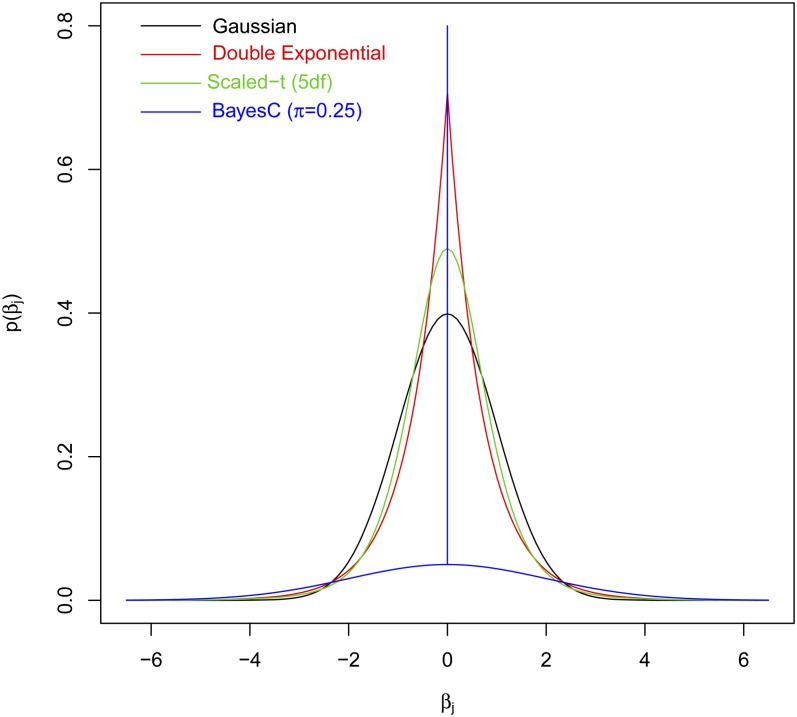
\includegraphics[width=8cm]{./Images/BGLR.jpg}
  \centering
  \caption{Figure \ref{fig:BGLR} by Perez et al.\cite{perez_genome-wide_2014} shows different prior densities implemented in BGLR}
  \label{fig:BGLR}
\end{figure}

\begin{figure}[h!]
  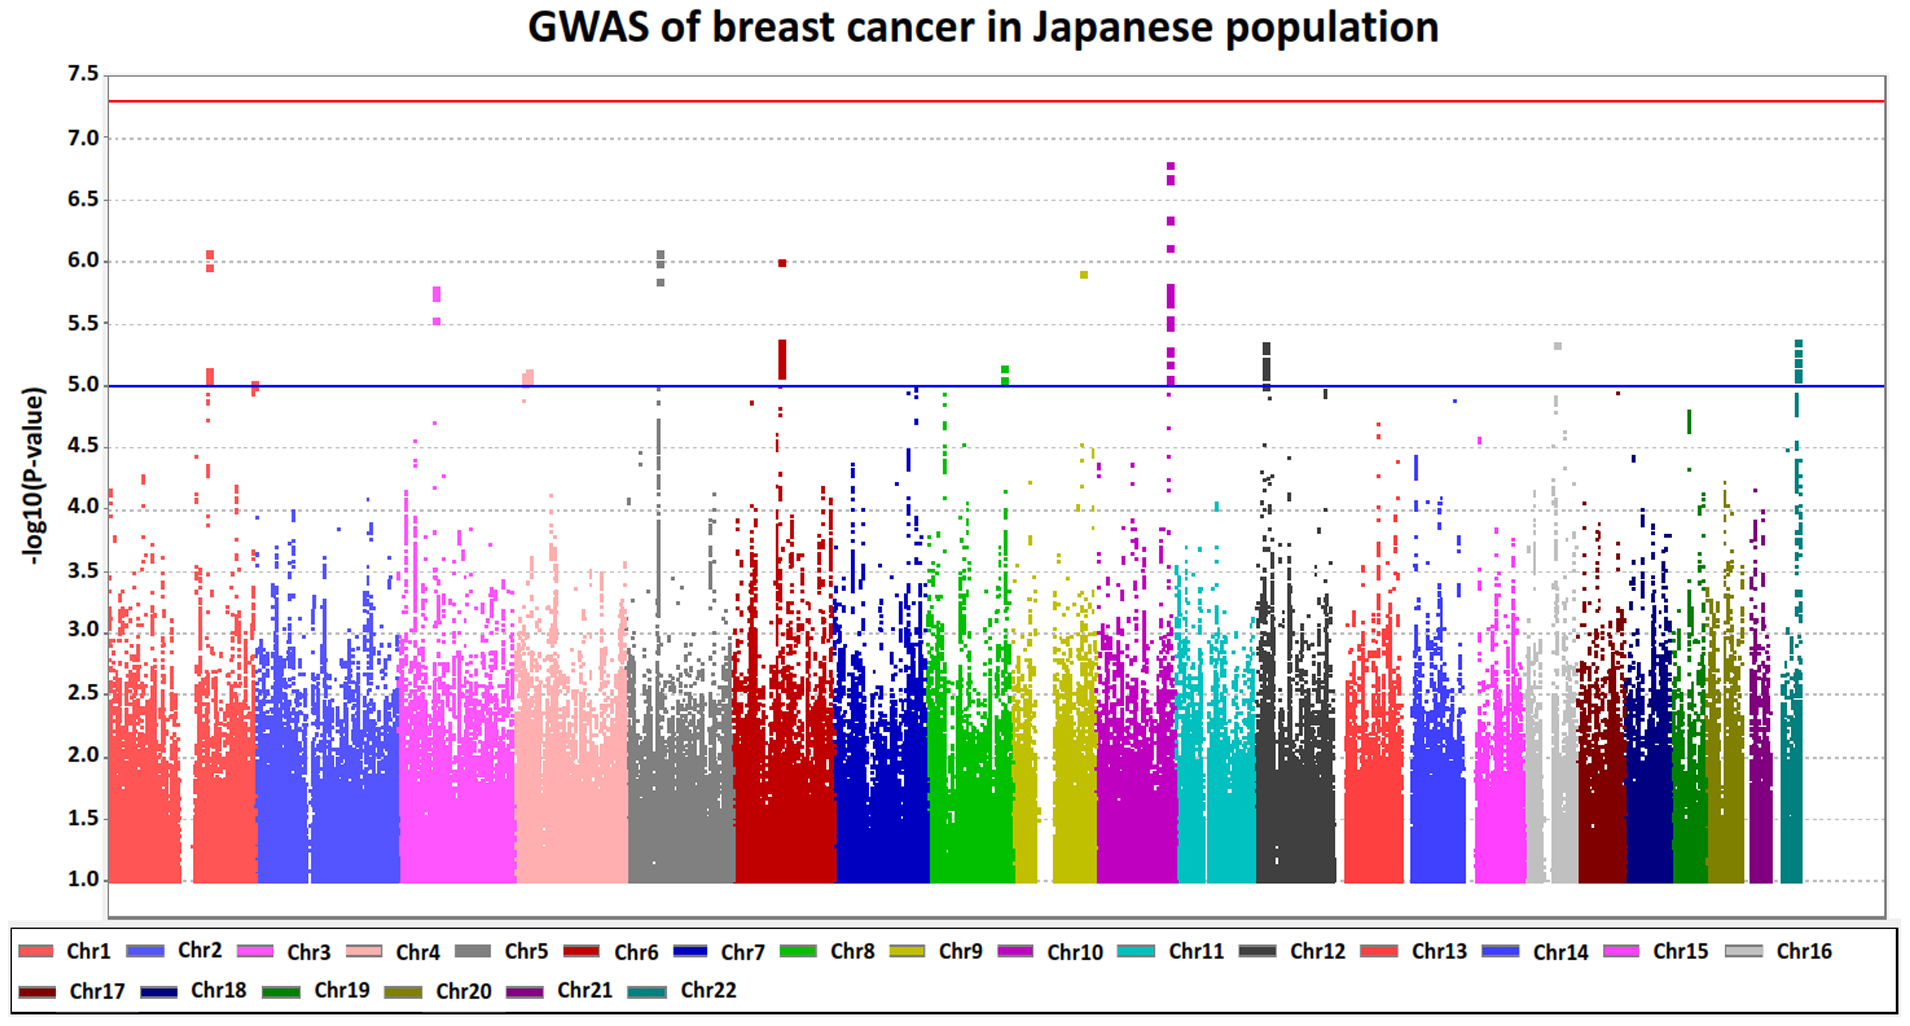
\includegraphics[width=8cm]{./Images/manhattan_plot.png}
  \centering
  \caption{Figure \ref{fig:manhattan1} shows an example manhattan plot by Low et al.\cite{low_genome-wide_2013} constructed from single marker regression across the genome. The y-axis is
  the $ -log(pvalue) $ and the x-axis contains SNP positions colored by chromosome.}
  \label{fig:manhattan1}
\end{figure}


\section{Related Work}

There is considerable literature in statistical learning approaches towards the analysis of GWAS data. Earlier work has
touched upon single marker regression methods and the whole host of approaches that can be applied to
deal with the multiple-testing issues.

Penalized regression methods such as ridge regression,\cite{austin_penalized_2013}
variable selection methods such as the lasso  and dimensionality reducing approaches such as principal components \cite{price_principal_2006} have all been applied and studied extensively in the analysis of
genome-wide data.

The discovery of gene-gene interactions is an active area of research where machine learning tools are being extensively employed \cite{upstill-goddard_machine_2013}
Bayesian methods and mixed models approaches within specific communities such as animal breeding have been
studied and applied for a long time, and are increasingly being used with genome-wide data. \cite{de_los_campos_whole-genome_2013}.

The issue of missing heritability and multi-factorial traits have gotten considerable attention in the literature. Multi-omics approaches toward improving prediction accuracy
are starting to gain traction with increase in the availability of computational resources. In addition to better prediction, these approaches can be particularly illuminating when
it comes to the biological mechanisms being studied. \cite{kim_multi-omics_2016}
An example would be to try and understand how much of the variation in the trait of interest can be explained by epigenetic variation, and is one of the things we are interested in here.

Another direction in the literature makes use of the methods mentioned so far to better understand the pathogenetic etiology of disease by studying genetic overlap between the disease and it's comorbidites.


\section{Data Description}

This project will require the use of heterogenous data types. The Genotyping information is stored as binary files, which needs to be accessed by a custom script
which reads information from metadata associated with the file. The large amount of data collected from a study of this size are organized by filename in a study manifest. Finding and collecting together the requisite data is itself
a challenge and needs to be done systematically.

Phenotypes are stored and organized by study cohort, examination number and consent group.
Variable checks need to be done before such data is extracted to ensure the right variables are present.
Demographic information is stored seperately and are also organized the same way.
We also incorporate Pedigree information into the analysis, which can be though of as a directed graph representing strengths of relationships between individuals.

Finally, methylation data needs to be extracted and incorporated into the analysis. I am still at the stage of validating this information, and will report further progress in the final report.

\section{Project Milestones}

This section will detail milestones so that I can roughly organize my work
toward the completion of this project. I am at the post Data-Extraction and Cleaning stage.
This step took some time as there are multiple different data types ( Genotypes, Phenotypes, Demographic, Methylation and Pedigree).
These include different consent groups, binary files, metadata, and data manifests.

\subsection{Completed Milestones}

\begin{itemize}
\item Prepare a proposal and survey important literature.
\item Dig deeper into the literature and search for implementational details.
\item Identify relevant software. R package BGLR will be used extensively to implement computationally intensive Bayesian methods.
\item Extract the data based on file-name lookup on study manifest file.
\item Clean, organize and explore the data. Include or remove clinical covariates as necessary.
\item Obtain metadata required for reading Binary files. This required searching the Affymetrix website for the corresponding genotyping array and the marker information.
\item Read in the Binary Genotype files and prepare the relationship matrices. This step was computationally intensive and the MSU High Performance Computing Cluster was used to prepare the relationship matrices.
The Relationship matrix was computed as \begin{equation}
R = XX^T
\end{equation}
Where $X$ is a high dimensional $9000*50000$ matrix containing marker information. More details on the role of the relationship matrix in inference will follow in the final project report.
\item Prepare a second draft with a detailed introduction and some results based on exploration.
\end{itemize}

\subsection{Remaining Milestones}

\begin{itemize}
\item Prepare the code, run and test it extensively on example data. Decide if simulations will be necessary.
\item Run the alogrithms on the Framingham data set, and collect the results. Prepare summaries and visualizations.
\item Prepare Final Report
\end{itemize}

\bibliography{cse_847_2}
\bibliographystyle{unsrt}
\end{document}
